% This is samplepaper.tex, a sample chapter demonstrating the
% LLNCS macro package for Springer Computer Science proceedings;
% Version 2.20 of 2017/10/04
%
\documentclass{llncs}
\pagestyle{empty}
\bibliographystyle{splncs04}
\setcounter{tocdepth}{2}
\makeatletter
\renewcommand*\l@author[2]{}
\renewcommand*\l@title[2]{}
\makeatletter
\usepackage[bookmarks]{hyperref}
%
\usepackage{graphicx}
\usepackage{minted}
\usepackage{longtable}
% If you use the hyperref package, please uncomment the following line
% to display URLs in blue roman font according to Springer's eBook style:
\renewcommand\UrlFont{\color{blue}\rmfamily}
\newcommand{\hs}{\mintinline{haskell}}
\usepackage{wrapfig}
\usepackage{todonotes}

\begin{document}
%
\title{Concurrency Oracles for Free}

%\titlerunning{Abbreviated paper title}
% If the paper title is too long for the running head, you can set
% an abbreviated paper title here
%
\author{Georgy Lukyanov \and Andrey Mokhov}
%
% \authorrunning{F. Author et al.}
% First names are abbreviated in the running head.
% If there are more than two authors, 'et al.' is used.
%
\institute{School of Engineering, Newcastle University, United Kingdom}

\maketitle

\begin{abstract}
This paper presents an approach to deriving \emph{concurrency oracles} for
processor instructions whose behaviour is formally specified using a state
transformer semantics. The presented approach does not require any modification
of the existing semantics, nor does it rely on writing a parser for the language
in which the semantics is described, thus justifying the ``for free'' part of
the title.

The main tool in our arsenal is \emph{ad-hoc polymorphism}: the presented
approach is only applicable when the semantics of processor instructions is
expressed using state transformation functions that can be reinterpreted in
different contexts. As we show in the paper, such semantics can be interpreted
not only for instruction simulation or verification, but also for extracting the
information about instruction dependencies, thus allowing us to identify
concurrency as well as various types of conflicts between instructions or blocks
of instructions.

\keywords{concurrency oracle
\and instruction set architecture
\and functional programming
\and polymorphism}
\end{abstract}
% \tableofcontents

\section{Introduction and motivation\label{sec:intro}}
Deciding whether two given events in a trace are \emph{concurrent}, i.e. have
no causal or data dependencies between them, is a major problem in the process
discovery field~\cite{2011_aalst_book}. Various methods for concurrency
extraction, often referred to as \emph{concurrency oracles}, have been
introduced, including the classic $\alpha$-algorithm~\cite{van2004workflow}, as
well as a few less widely known methods, e.g. see~\cite{cook1998event},
\cite{mokhov2016mining} and the review paper~\cite{augusto2017automated}. A
good example of treating a concurrency oracle as a self-contained problem can
be found in~\cite{dumas2015process}.

In this paper we present an approach for deriving concurrency oracles for
events that correspond to processor instructions and blocks of instructions. The
input to the proposed approach is the \emph{microarchitectural semantics} of
instructions, which gives a precise description of how an instruction execution
changes the state of the processor.

A popular method to describe microarchitectural semantics is to use a dedicated
domain-specific language embedded in a high-level general-purpose host language,
such as Haskell or Coq. Two pioneering works in this domain
are~\cite{fox2010trustworthy}, where the Arm v7 instruction set architecture
is formalised in HOL4, and~\cite{kennedy2013coq}, where x86 architecture is
formalised in Coq.

The authors of this paper have also used an embedded domain-specific language
to describe the semantics of a space-grade
microarchitecture~\cite{mokhov2018formal}. In particular, it was demonstrated
that the same semantics can be reused in different contexts: to simulate the
processor and to perform formal verification of programs executed by the
processor. In this paper we take this work further, by demonstrating that the
very same semantics can be reused for deriving concurrency oracles that given
two instructions, or blocks of instructions, can determine whether they are
concurrent and, if not, report the data dependency conflicts.

We start by studying several common examples of processor instructions, noticing
that different instructions require different features from the language used to
describe them; see~\S\ref{sec:instructions}. We proceed by introducing the
language for specifying semantics in more detail and then describe the semantics
of a small instruction set (\S\ref{sec:metalanguage}). The approach to deriving
concurrency oracles is presented in~\S\ref{sec:oracles}, followed by a
discussion.


\vspace{-1mm}
\section{Instruction set architecture semantics\label{sec:instructions}}
\vspace{-2mm}
In this section we introduce the computational metalanguage by example. We will
use the metalanguage to describe the semantics of a part of a simple generic instruction
set architecture. The later sections will introduce a formal definition of the
metalanguage, instruction and program semantics and present a method of extracting static
data dependencies of instructions with certain properties from the semantic definitions
leading to a construction of a~\emph{concurrent oracle}.

\begin{figure}[H]
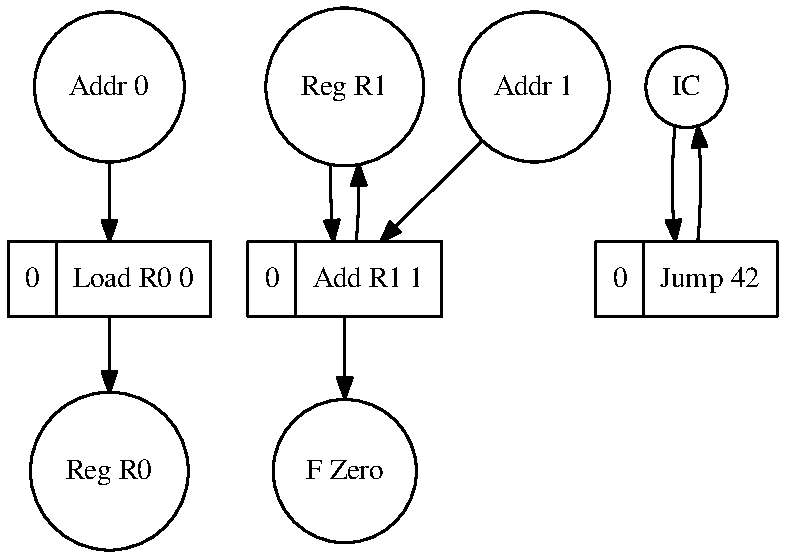
\includegraphics[width=35em]{img/loadJumpAdd.pdf}
\caption{Static data dependencies of~\hs{Load R0 0},~\hs{Add R1 1} and~\hs{Jump 42} instructions.}
\end{figure}

\subsubsection{Unconstrained semantics. Load} Literally every real-world instruction set include an instruction
which loads a data word from a memory location to a register. Here is how the
semantics of such an instruction can be encoded in the metalanguage:

\begin{minted}{haskell}
load reg addr = \read write -> Just $
    write (Reg reg) (read (Addr addr))
\end{minted}

In this definition we use two metalanguage terms:~\hs{read} and~\hs{write} to encode
the behaviour. These terms are polymorphic effectful functions with the following
types:

\begin{minted}{haskell}
read :: MachineKey -> f Word64
read =

write :: MachineKey -> f Word64 -> f ()
write =
\end{minted}

The~\hs{read} term queries the microarchitectural state for the value of a key and
returns it wrapped in a context~\hs{f}, which is, in fact, the reason for the
metalanguage to be~\emph{polymorphic}. In this case the context~\hs{f} may be any
type constructor of kind~\hs{* -> *}. However, not every instruction semantics may
be expressed in an unconstrained context. Let us consider semantics of some other
instructions to elaborate more on the nature of~\hs{f}.

\subsubsection{Functorial semantics. Jump}

Another popular instruction is the unconditional control flow transfer:

\begin{minted}{haskell}
jump offset = \read write -> Just $
    write IC ((+ offset) <$> (read IC))
\end{minted}

The semantics of this instruction increments the instruction counter~\hs{IC}
to transfer the control to another instruction in the program. This definition
has an crucial difference from~\hs{load}: it uses
the~\hs{<$>}\footnote{Function~\hs{<$>} (pronounced "fmap") of type
\hs{Functor f => (a -> b) -> f a -> f b} allows to transform the values in an
computational context with a pure function.} function of the~\hs{Functor} type
class, thus restricting~\hs{f} to be a~\hs{Functor}:

\begin{minted}{haskell}
read :: Functor f => MachineKey -> f Word64
read =

write :: Functor f => MachineKey -> f Word64 -> f ()
write =
\end{minted}

In this definition functorial constraint is required to apply the increment function
~\hs{(+ offset) :: Num a => a -> a} to the instruction counter enclosed in a computational
context~\hs{f}.

Later in the paper we will instantiate~\hs{f} as a context of data dependency
tracking. It turns out that the~\hs{Functor} constraint is equivalent to stating
that a computation may have at most one static dependency, being the instruction
counter in the case of~\hs{load}.

\subsubsection{Applicative semantics. Add}

The~\hs{add} instruction semantics performs the addition of the values of
a register and a memory cell. If the result of the addition is equal to zero,
the semantics sets the~\hs{Zero} microarchitectural flag~\hs{True}, or to~\hs{False} otherwise.

The Haskell definition of the semantic function is a bit more involved than the previous
ones. It turns out that the~\hs{Functor} context is not expressive enough and a
more powerful abstraction is needed. The following definition of~\hs{add} requires
\hs{f} to be at least an~\hs{Applicative}:

\begin{minted}{haskell}
add reg addr = \read write -> Just $
    let result = (+)    <$> read (Reg reg) <*> read (Addr addr)
        isZero = (== 0) <$> result
    in  write (Reg reg) result *>
        write (F Zero)  isZero
\end{minted}

Let us describe what is going on here. The definition may be broken down in three
classes of actions: reading data, processing it on-the-fly and writing data back in the store.

The first~\hs{let}-binding uses~\hs{Applicative} notation
to read the values from the register and memory address and add them up. Note that
this notation is~\emph{declarative}, hence it rather states that the~\hs{result}
is supposed to be a sum of values of two entities than performs actual computation.
This intuition is very important for understanding the static dependency tracking semantics
of instructions:~\hs{Reg reg} and~\hs{Addr addr} are declared as static input dependencies of
the~\hs{add} instruction. However, since the semantics may be executed in any~\hs{Applicative} context,
this dependency-tracking inspired intuition must not
obscure other possible interpretations of the semantics. For instance, in a stateful
simulation context, the~\hs{result} will be computed based on concrete data values
read from the underlying store.

The second line of the~\hs{let}-binding is quite similar to the expression in the
semantics of the~\hs{jump} instruction. The type of the~\hs{result} is~\hs{f Word64},
hence the zero testing function~\hs{(==) 0} of type~\hs{(Num a, Eq a) => a -> Bool}
must be mapped over the context~\hs{f} with~\hs{<$>} to obtain the value of type
\hs{f Bool}.

The latter two lines of the definition perform two~\hs{write} operations chained with
the applicative notation combinator~\hs{*>} of type~\hs{Applicative f => f a -> f b -> f b}.
This declares the values~\hs{Reg reg} and~\hs{F Zero} to be output dependencies of
the computation and that the writes mush be both performed.

An interesting feature of the~\hs{Applicative} notation is that it does not specify the exact order of
performing actions. This feature is useful in embedded domain-specific languages
with concurrency, for instance Facebook's Haxl~\cite{Marlow:2014:NFA:2692915.2628144}.

\hs{Applicative} functors are powerful enough to express the semantics of a
large class of instructions. In this paper we exploit their features to not only
specify the execution semantics but also automatically track static data dependencies
of instructions. However not every instruction of modern architecture may be
equipped with~\hs{Applicative} semantics. If the behaviour start to depend on the
actual data, i.e.~\emph{dynamic} data dependencies emerge, the semantics can not
be encoded using an~\hs{Applicative}. A more powerful abstraction is required.

\subsubsection{Monadic semantics. Memory indirect Load}

The indirect memory access instruction looks up a value in a memory cell and uses
it as the effective address in the regular load instruction. Since the effective
address can not be determined statically in the general case, this instruction
has a dynamic data dependency. The polymorphic computational metalanguage requires
the context~\hs{f} to be a~\hs{Monad} in order to be able to encode such behaviour.
Consider the definition of the semantics of the~\hs{loadMI} instruction, which
uses Haskell monadic ~\hs{do}-notation:

\begin{minted}{haskell}
loadMI reg addr read write = Just $ do
    addr' <- read (Addr addr)
    write (Reg reg) (read (Addr addr'))
\end{minted}

The first line extracts the effective address from the monadic context
and binds the identifier~\hs{addr'} to it. Here is the catch: expressions
on left-hand-side and right-hand-side of the~\hs{<-} symbol have different types.
The~\hs{read (Addr addr)} is of type~\hs{Monad f => f MemoryAddress} and the
identifier~\hs{addr'} has type \hs{MemoryAddress}. The main feature of~\hs{Monad}
is ability to extract a value from an effectful context and pass it in the further
computation as it was pure. This gives us a possibility to pass the~\hs{addr'}
as an argument to the next~\hs{read} operation.

Monadic semantics is more powerful that unconstrained, functorial and applicative ones,
but we are no more able to extract all the dependencies of the computation if
\hs{f} is restricted to~\hs{Monad}, since some of them will not be static. Therefore,
concurrency oracles can not be built for~\hs{Monad}-flavoured computations.

We have given examples of four kinds of semantic computations: unrestricted, functorial,
applicative and monadic. In every definition we used functions~\hs{read} and~\hs{write}
and have constrained the context~\hs{f} with~\hs{Functor},~\hs{Applicative}
or~\hs{Monad}. The resulting types of~\hs{read} and~\hs{write} follow a certain
pattern, which may be encoded in the Haskell type system. In fact, a generic
~\hs{read} may be assigned with type~\hs{forall c. MachineKey -> (c f) Word64} and
generic~\hs{write} with~\hs{forall c. MachineKey -> (c f) Word64 -> (c f) ()}. Here,
type variable~\hs{c} mush have kind~\hs{* -> Constraint}. This allows to instantiate
~\hs{c} with~\hs{Functor}, \hs{Applicative}, \hs{Monad} or any other suitable constraint,
thus making the metalanguage polymorphic in the computational context.

The next section will present a formal definition of the metalanguage, instruction
and program semantics. The section~\ref{oracles} will describe the construction of
concurrency oracles for programs comprising unrestricted, functorial, applicative,
but not monadic instructions.



\section{Polymorphic computational metalanguage\label{sec:metalanguage}}

In the previous section we have described the semantics of several instructions of
a generic computer architecture in terms of a polymorphic computational metalanguage.
This section presents the formal definition of the metalanguage and provides a more
formal description of the instruction and program semantics.

\textbf{A remark on formal definitions}
Before we start, let us make a remark on what we consider a formal definition.
We do not aim to formalise our tools in any kind of foundational mathematical system,
such as ZF\footnote{Zermelo-Fraenkel set theory.} or homotopy type theory. We are
presenting an elegant way of solving a well-known problem and we use the Haskell
programming language to implement the solution. Therefore, we consider a concept
to be~\emph{formally} defined if it is expressed as a Haskell data type. This may
sound hand-wavy, but since Haskell has a static type system (a variant of
System~F~\cite{Sulzmann:2007:SFT:1190315.1190324}) and operational semantics, we
can be formal enough.

\textbf{Definition (polymorphic computational metalanguage):\label{def:metalanguage}}
A term of the metalanguage is a value of the following Haskell type:

\begin{minted}[xleftmargin=10pt]{haskell}
type Semantics c a =
    forall f. c f => (Key -> f Value)
                  -> (Key -> f Value -> f ())
                  -> Maybe (f a)
\end{minted}

\noindent A~\hs{Semantics} is essentially a rank-2 polymorphic\footnote{A rank-2 polymorphic
function is one taking as a parameter another function, which is in turn (rank-1)
polymorphic. This feature requires the~\hs{RankNTypes} language extension of the
Glasgow Haskell Compiler.}
effectful computation depending on two functions,
which we will usually refer to as~\hs{read} and~\hs{write}.

Let us now give some intuition for the components of the metalanguage.
The~\hs{Semantics c a}
type may be thought as a mutable dictionary. The~\hs{read} function has
type~\hs{Key -> f Value} --- it takes
a key and gives back an effectful value looked up in the dictionary. The~\hs{write}
function takes a key and an effectful value and alters the value of the key in
the dictionary. The semantics can be partial, hence the the return type~\hs{f a}
is wrapped in the \hs{Maybe} type constructor.
\hs{Maybe}\footnote{Defined in the Haskell's \textsf{base} library as~\hs{data Maybe a = Just a | Nothing}.}
is an idiomatic Haskell encoding of partial definitions. The semantics may
become partial if we, for example, fix the constraint type variable~\hs{c}
to~\hs{Applicative}, thus losing the possibility to encode the monadic
components of the instruction set. \hs{Maybe} allows us to treat such
partially-defined semantics in a safe and formal way.

\textbf{Definition (Instruction Set):} An~\emph{instruction set} is an algebraic
data type with as many data constructors as there are instructions.
If an instruction has an argument, it is defined as an argument of the
corresponding data constructor.

Consider an example definition of an instruction set consisting
of instructions described in the previous sections and the related auxiliary types:

\begin{minted}[xleftmargin=10pt]{haskell}
data Instruction = Load   Register MemoryAddress
                 | LoadMI Register MemoryAddress
                 | Add    Register MemoryAddress
                 | Jump   Value

data Register = R0 | R1 | R2 | R3

type MemoryAddress = Value
\end{minted}

\noindent
\textbf{Definition (Instruction Set Semantics):}
The \emph{semantics of an instruction set} is a Haskell function mapping
data constructors of the instruction set to the terms of the polymorphic
computational metalanguage.

The definition of an instruction set semantics is the point where the metalanguage
has to be made monomorphic, i.e. the context constraint has to be instantiated with
a concrete one. Below we present unrestricted, functorial, applicative and
monadic semantics for the defined instruction set.

We start from the~\hs{Load} instruction which may be executed in any
context\footnote{The~\hs{Unrestricted} constraint is not exactly idiomatic Haskell and
requires some tricks to be defined.}:

\vspace{-1mm}
\begin{minted}[xleftmargin=10pt]{haskell}
semanticsU :: Instruction -> Semantics Unrestricted ()
semanticsU (Load reg addr) = load reg addr
semanticsU _               = const (const Nothing)
\end{minted}

Note that the Haskell wildcard pattern `\hs{_}' is used to match all instructions
that require a more restrictive context. The~\hs{const (}\hs{const Nothing)} expression
is equivalent to~\hs{\read write -> Nothing} and constructs a stub for these
more restricted semantics. The function \hs{load} has been defined
in~\S\ref{sec:instructions}.

The instantiation of~\hs{c} with a~\hs{Functor} allows us to implement the
semantics of the instruction~\hs{Jump}:

\begin{minted}[xleftmargin=10pt]{haskell}
semanticsF :: Instruction -> Semantics Functor ()
semanticsF (Jump simm) = jump simm
semanticsF i           = semanticU i
\end{minted}

\noindent Here we use the definition of \hs{jump} from~\S\ref{sec:instructions}
and fall back to unrestricted semantics definition \hs{semanticU} for
the~\hs{Load} instruction, hence avoiding code duplication.

The remaining definitions are analogous:

\begin{minted}[xleftmargin=10pt]{haskell}
semanticsA :: Instruction -> Semantics Applicative ()
semanticsA (Add reg addr) = add reg addr
semanticsA i              = semanticsF i

semanticsM :: Instruction -> Semantics Monad ()
semanticsM (LoadMI reg addr) = loadMI reg addr
semanticsM i                 = semanticsA i
\end{minted}

We can now define the semantics of a block of instructions by reducing
a given list of instructions:

\begin{minted}[xleftmargin=10pt]{haskell}
blockSemanticsA :: [Instruction] -> Semantics Applicative ()
blockSemanticsA xs = \r w ->
    foldr (\x acc -> (*>) <$> acc <*> semanticsA x r w) nop xs
    where nop = Just $ pure ()
\end{minted}

\noindent The semantics of an empty block is~\hs{nop} (i.e. a \emph{no-op}
instruction). The semantics of a non-empty list is the semantics of its head
chained with the semantics of the tail. We need to lift the applicative chaining
operation since the~\hs{Maybe} type constructor also is an instance
of~\hs{Applicative} and the behaviour of~\hs{*>} returns the contents of the
last~\hs{Just}, which is would be wrong.

Now, with the instruction semantics defined in terms of the polymorphic
computational metalanguage, we may proceed to evaluating the metalanguage
in concrete contexts to get a practical interpretation of the instruction set.

The next section presents the interpretation of unrestricted, functorial and
applicative instructions yielding concurrency oracles for programs.

Other interpretations of the metalanguage are also possible. In the technical
report~\cite{mokhov2018formal} we present a formal model of a processor
developed for space missions, where we use a more restricted, monadic
metalanguage, making emphasis on symbolic program execution and automated
theorem proving: the framework allows to verify functional properties of
programs and automatically check if two programs are semantically equivalent.
The metalanguage presented in this paper also allows these interpretations,
but the focus of this paper is different: automated derivation of concurrency
oracles.

\section{Concurrency oracles\label{sec:oracles}}
In this section we present a method to derive concurrency oracles from the instruction
semantics encoded in the  metalanguage (Definition~\ref{def:metalanguage}).
More specifically, we aim to reason about instructions that
have only \emph{static dependencies}.

We start by introducing formal definitions and Haskell encodings of the concepts
required for building concurrency oracles.
First, we define the notions of input and output dependencies of a computation.

\textbf{Definition (input dependency):\label{def:in-dependencies}}
Consider a term $f$ of an applicative metalanguage~\hs{Semantics Applicative a}.
A key $k$ is an~\emph{input dependency} of the term $f$ if the term $f$
performs a~\hs{read} of the key $k$.

\textbf{Definition (output dependency):\label{def:out-dependencies}}
Consider a term $f$ of an applicative metalanguage~\hs{Semantics Applicative a}.
A key $k$ is an~\emph{output dependency} of the term $f$ if the term $f$
performs a~\hs{write} of the key $k$.

\textbf{Definition (dependencies):\label{def:dependencies}}
Consider a term $f$ of an applicative metalanguage~\hs{Semantics Applicative a}.
The~\emph{dependencies} of the term $f$ are a pair of sets $I$ and $O$,
comprising the input and output dependencies of the term $f$, respectively.

In the Haskell implementation, we do not distinguish between input and output dependencies
in the type level, thus the function determining the dependencies of a computation
has the following type:

\begin{minted}[xleftmargin=10pt]{haskell}
dependencies :: Semantics Applicative a -> Maybe ([Key], [Key])
\end{minted}

\noindent
The~\hs{Maybe} type constructor comes from the definition of the metalanguage:
if the applicative semantics is partial (returns~\hs{Nothing}) it is impossible
to extract its static dependencies. Successful static analysis yields a pair of
lists representing the sets of input and output dependencies of a computation.

To extract the static data dependencies of an applicative computation we need to
interpret its semantics in the special context of a \emph{constant functor}.

\subsection{The constant functor}

The~\hs{Const a b} data type is defined as follows~\cite{Mcbride:2008:APE:1348940.1348941}:

\begin{minted}[xleftmargin=10pt]{haskell}
newtype Const a b = Const { getConst :: a }
\end{minted}

\noindent
A value of the~\hs{Const a b} is just a value of any type~\hs{a}
wrapped in a data constructor. However, it is important that the type constructor
has a~\emph{phantom type} variable. This type variable allows us to
declare useful instances of standard Haskell type classes such as~\hs{Functor}
and \hs{Applicative} for \hs{Const a}. We would like to use this data type as a
computational context for applicative semantics, hence we declare the
corresponding instance\footnote{\hs{Const a} also has a \hs{Functor} instance,
where~\hs{fmap _ (Const x) = Const x}}:

\begin{minted}[xleftmargin=10pt]{haskell}
instance Monoid m => Applicative (Const m) where
    pure _              = Const mempty
    Const x <*> Const y = Const (x `mappend` y)
\end{minted}

This instance exactly describes the desired behaviour of static dependency tracking
computational context.~\hs{Const [Key]} is an applicative functor that ignores
its enclosed value, but accumulates the declared dependencies using the~\hs{Monoid}
instance for Haskell list data type\footnote{The empty list~\hs{[]} is the
neutral element and the list concatenation~\hs{(++)} is the associative binary operation}.

\subsection{Extracting dependencies}

Using the elegant~\hs{Const a b} abstraction we define the \hs{dependencies} function:

\begin{minted}[xleftmargin=10pt]{haskell}
dependencies :: Semantics Applicative a -> Maybe ([Key], [Key])
dependencies s = partitionEithers . getConst <$> s read write
  where read  k    =       Const [Left  k]
        write k fv = fv *> Const [Right k]
\end{minted}

\noindent
We instantiate the polymorphic computation context with \hs{f = Const [Key]}
and supply custom tracking \hs{read} and \hs{write} functions. In fact, \hs{read}
does not perform any reading and just tracks the key as an input dependency,
whereas \hs{write} tracks the key as an output dependency and executes the
effectful computation \hs{fv}, to appropriately track its dependencies. The
resulting list of keys gets unwrapped and unzipped by
\hs{partitionEithers}~\hs{.}~\hs{getConst}.

Now we are fully armed to define concurrency oracles for terms of the
applicative metalanguage.

\subsection{Concurrency oracle}
% \vspace{-2em}
A concurrency oracle is a function taking two computations and statically
determining if they are data~\emph{concurrent}, i.e. do not share any
data dependencies.


\textbf{Definition (Concurrency Oracle Answer):\label{def:concurrency-status}}
Two terms of the metalanguage are \emph{concurrent} if they do not share any
data dependencies. They are in a \emph{read} or \emph{write conflict} if they
share any input or output dependencies, respectively. If the share both input
and output dependencies then they are considered to be in a \emph{read-write
conflict}. We use the following data type is used to encode concurrency oracle
answers:

\begin{minted}[xleftmargin=10pt]{haskell}
data OracleAnswer k = Concurrent
                    | ReadConflict [k]
                    | WriteConflict [k]
                    | ReadWriteConflict [k]
\end{minted}

\textbf{Definition (concurrency oracle):\label{def:oracle}}
Consider two terms with applicative semantics $s1$ and $s2$ of
type~\hs{Semantics Applicative a}. A~\emph{concurrency oracle} is defined as the
Haskell function:
% \vspace{-3em}
\begin{minted}[xleftmargin=10pt]{haskell}
concurrencyOracle :: Eq k => Semantics Applicative k v1 a
                          -> Semantics Applicative k v2 a
                          -> Maybe (OracleAnswer k)
concurrencyOracle s1 s2 = do
    (r1, w1) <- dependencies s1
    (r2, w2) <- dependencies s2
    let readConflicts      = intersect r1 r2
        writeConflicts     = intersect w1 w2
        readWriteConflicts = intersect (r1 ++ w1) (r2 ++ w2)
    pure $ case (readConflicts, writeConflicts, readWriteConflicts) of
        ([], [], [] ) -> Concurrent
        (rs, [], rws) | rs == rws -> ReadConflict rs
        ([], ws, rws) | ws == rws -> WriteConflict ws
        (_ , _ , rws) -> ReadWriteConflict rws
\end{minted}
% \vspace{-3em}

The oracle determines static dependencies of two given terms and examines
several possible cases of the intersections of their input and output
dependencies.

\subsection{Example oracles}

In this subsection we show two examples to illustrate the usage of concurrency
oracles. The examples are given in the form of interactive sessions, where
`\hs{ghci>}' denotes the command prompt.

Two \hs{Load} instructions with different arguments are concurrent as confirmed
by the oracle returning the result \hs{Just Concurrent}:

\begin{minted}[xleftmargin=10pt]{haskell}
ghci> concurrencyOracle (semanticsA (Load R0 0))
                        (semanticsA (Load R1 1))
Just Concurrent
\end{minted}

\noindent
Extending the first computation with an additional \hs{Add} instruction causes
a read conflict:
\begin{minted}[xleftmargin=10pt]{haskell}
ghci> let p1 = blockSemanticsA [ Load R0 0
                               , Add  R0 1 ]
ghci> let p2 = semanticsA (Load R1 1))
ghci> concurrencyOracle
Just (ReadConflict [Addr 1])
\end{minted}
We can produce a graphical representation of dependencies between and
within programs \hs{p1} and \hs{p2} with the following commands:

\begin{minted}[xleftmargin=10pt]{haskell}
ghci> let g1 = programDataGraph (zip [0..] [Load R0 0, Add R0 1])
ghci> let g2 = programDataGraph (zip [0..] [Load R1 1])
ghci> drawGraph (overlay g1 g2)
\end{minted}

The resulting dependency graph is shown in Fig.~\ref{fig-example-graph}.
% In the graph, instructions labelled with 1 and 2 belong to the blocks~\hs{p1}
% and~\hs{p2} respectively.
As one can see, both computations share the register \hs{R0}, just like the
oracle has determined.

\begin{figure}
\vspace{-6mm}
\centerline{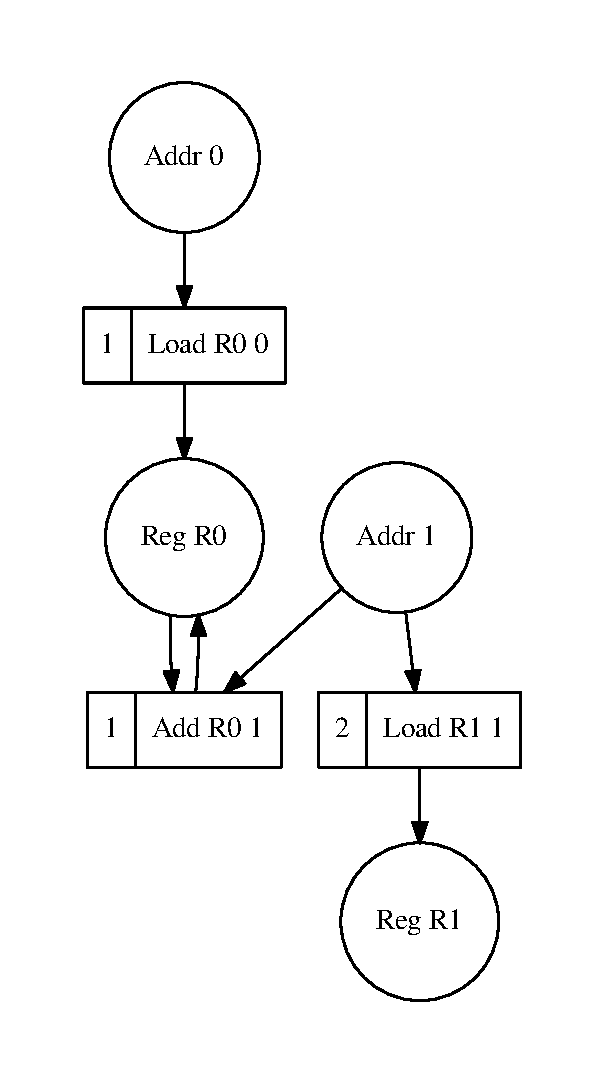
\includegraphics[scale=0.6]{img/oracle2.pdf}}
\vspace{-6mm}
\caption{An overlay of static dependency graphs of two blocks of instructions.\label{fig-example-graph}}
\vspace{-6mm}
\end{figure}


\section{Synthesis of efficient hardware microcontrollers\label{sec:scenarios}}
In this section, we present a tool for extracting~\emph{scenarios} from
blocks of instructions.~\todo{include scenario definition from Alessandro's journal paper
together with a reference.}

To mine scenarios from blocks of instructions, we partially reuse the methodology
used for construction of the concurrency oracles from the previous section. The methodology
involves calculating the set of static dependencies of the block of instructions,
constructing the~\emph{unfolded} static dependencies graph~\footnote{Similar to one in the
figure~\ref{fig-example-graph}, but with with data-vertexes duplicated on every update.};
and then wiping out the data-vertexes preserving the transitive connections
of instruction-vertexes. A~\emph{transitive closure} of the resulting graph will
display the partial order on the set of events represented as instruction-vertexes.
\todo{Make this a good-looking algorithm}.

Extraction of scenarios from programs enables us to use the associated methods for
compiling programs into application-specific hardware. The Conditional Partial
Order Graphs formalism enables synthesis of scenarios, allowing to compile them into
a circuit with some functionality shared.

\begin{figure}
\vspace{-4mm}
\centerline{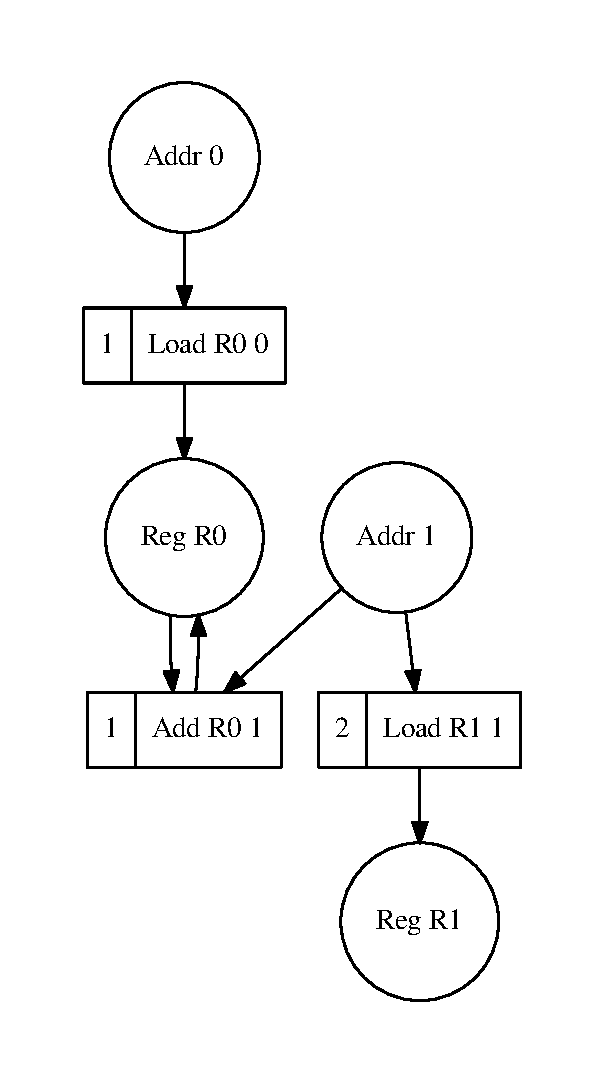
\includegraphics[scale=0.6]{img/oracle2.pdf}}
\vspace{-3mm}
\caption{An overlay of static dependency graphs of two blocks of instructions.\label{fig-example-graph}}
\vspace{-9mm}
\end{figure}

\section{Conclusion}
% \begin{wrapfigure}{r}{0.4\textwidth}
%   % \begin{center}
%     \vspace{-25mm}
%     \includegraphics[scale=0.4]{img/.pdf}
%   % \end{center}
%   \caption{Approximation of static dependencies of an array summation program.\label{fig-sum}}
% \end{wrapfigure}

% The metalanguage closely resembles state
% transformers.
The paper presented a metalanguage for describing the semantics of instruction
set architectures. Multiple interpretations of the metalanguage terms allow us
to evaluate the semantics in different contexts without its modification. As the
primary application, we present an approach to deriving concurrency oracles of
the instructions with only static data dependencies.

To handle instructions whose dependencies are dynamic, it is possible to use
conservative approximation of dependencies. For example, Fig.~\ref{fig-sum}
shows the dependency graph for a program implementing the Euclidean algorithm
for computing the greatest common divisor of two numbers that contains
a conditional branch instruction \hs{JumpZero}, which modifies the instruction
counter \hs{IC} only if the previous instruction set the \hs{Zero} flag. In this
example, we conservatively assume that \hs{JumpZero} always depends on \hs{IC}.
Our future work includes the application of the presented methodology to
extracting concurrency from real-world processor specifications, as described
in~\cite{mokhov2018formal}.

\vspace{-10mm}
\begin{figure}
\centerline{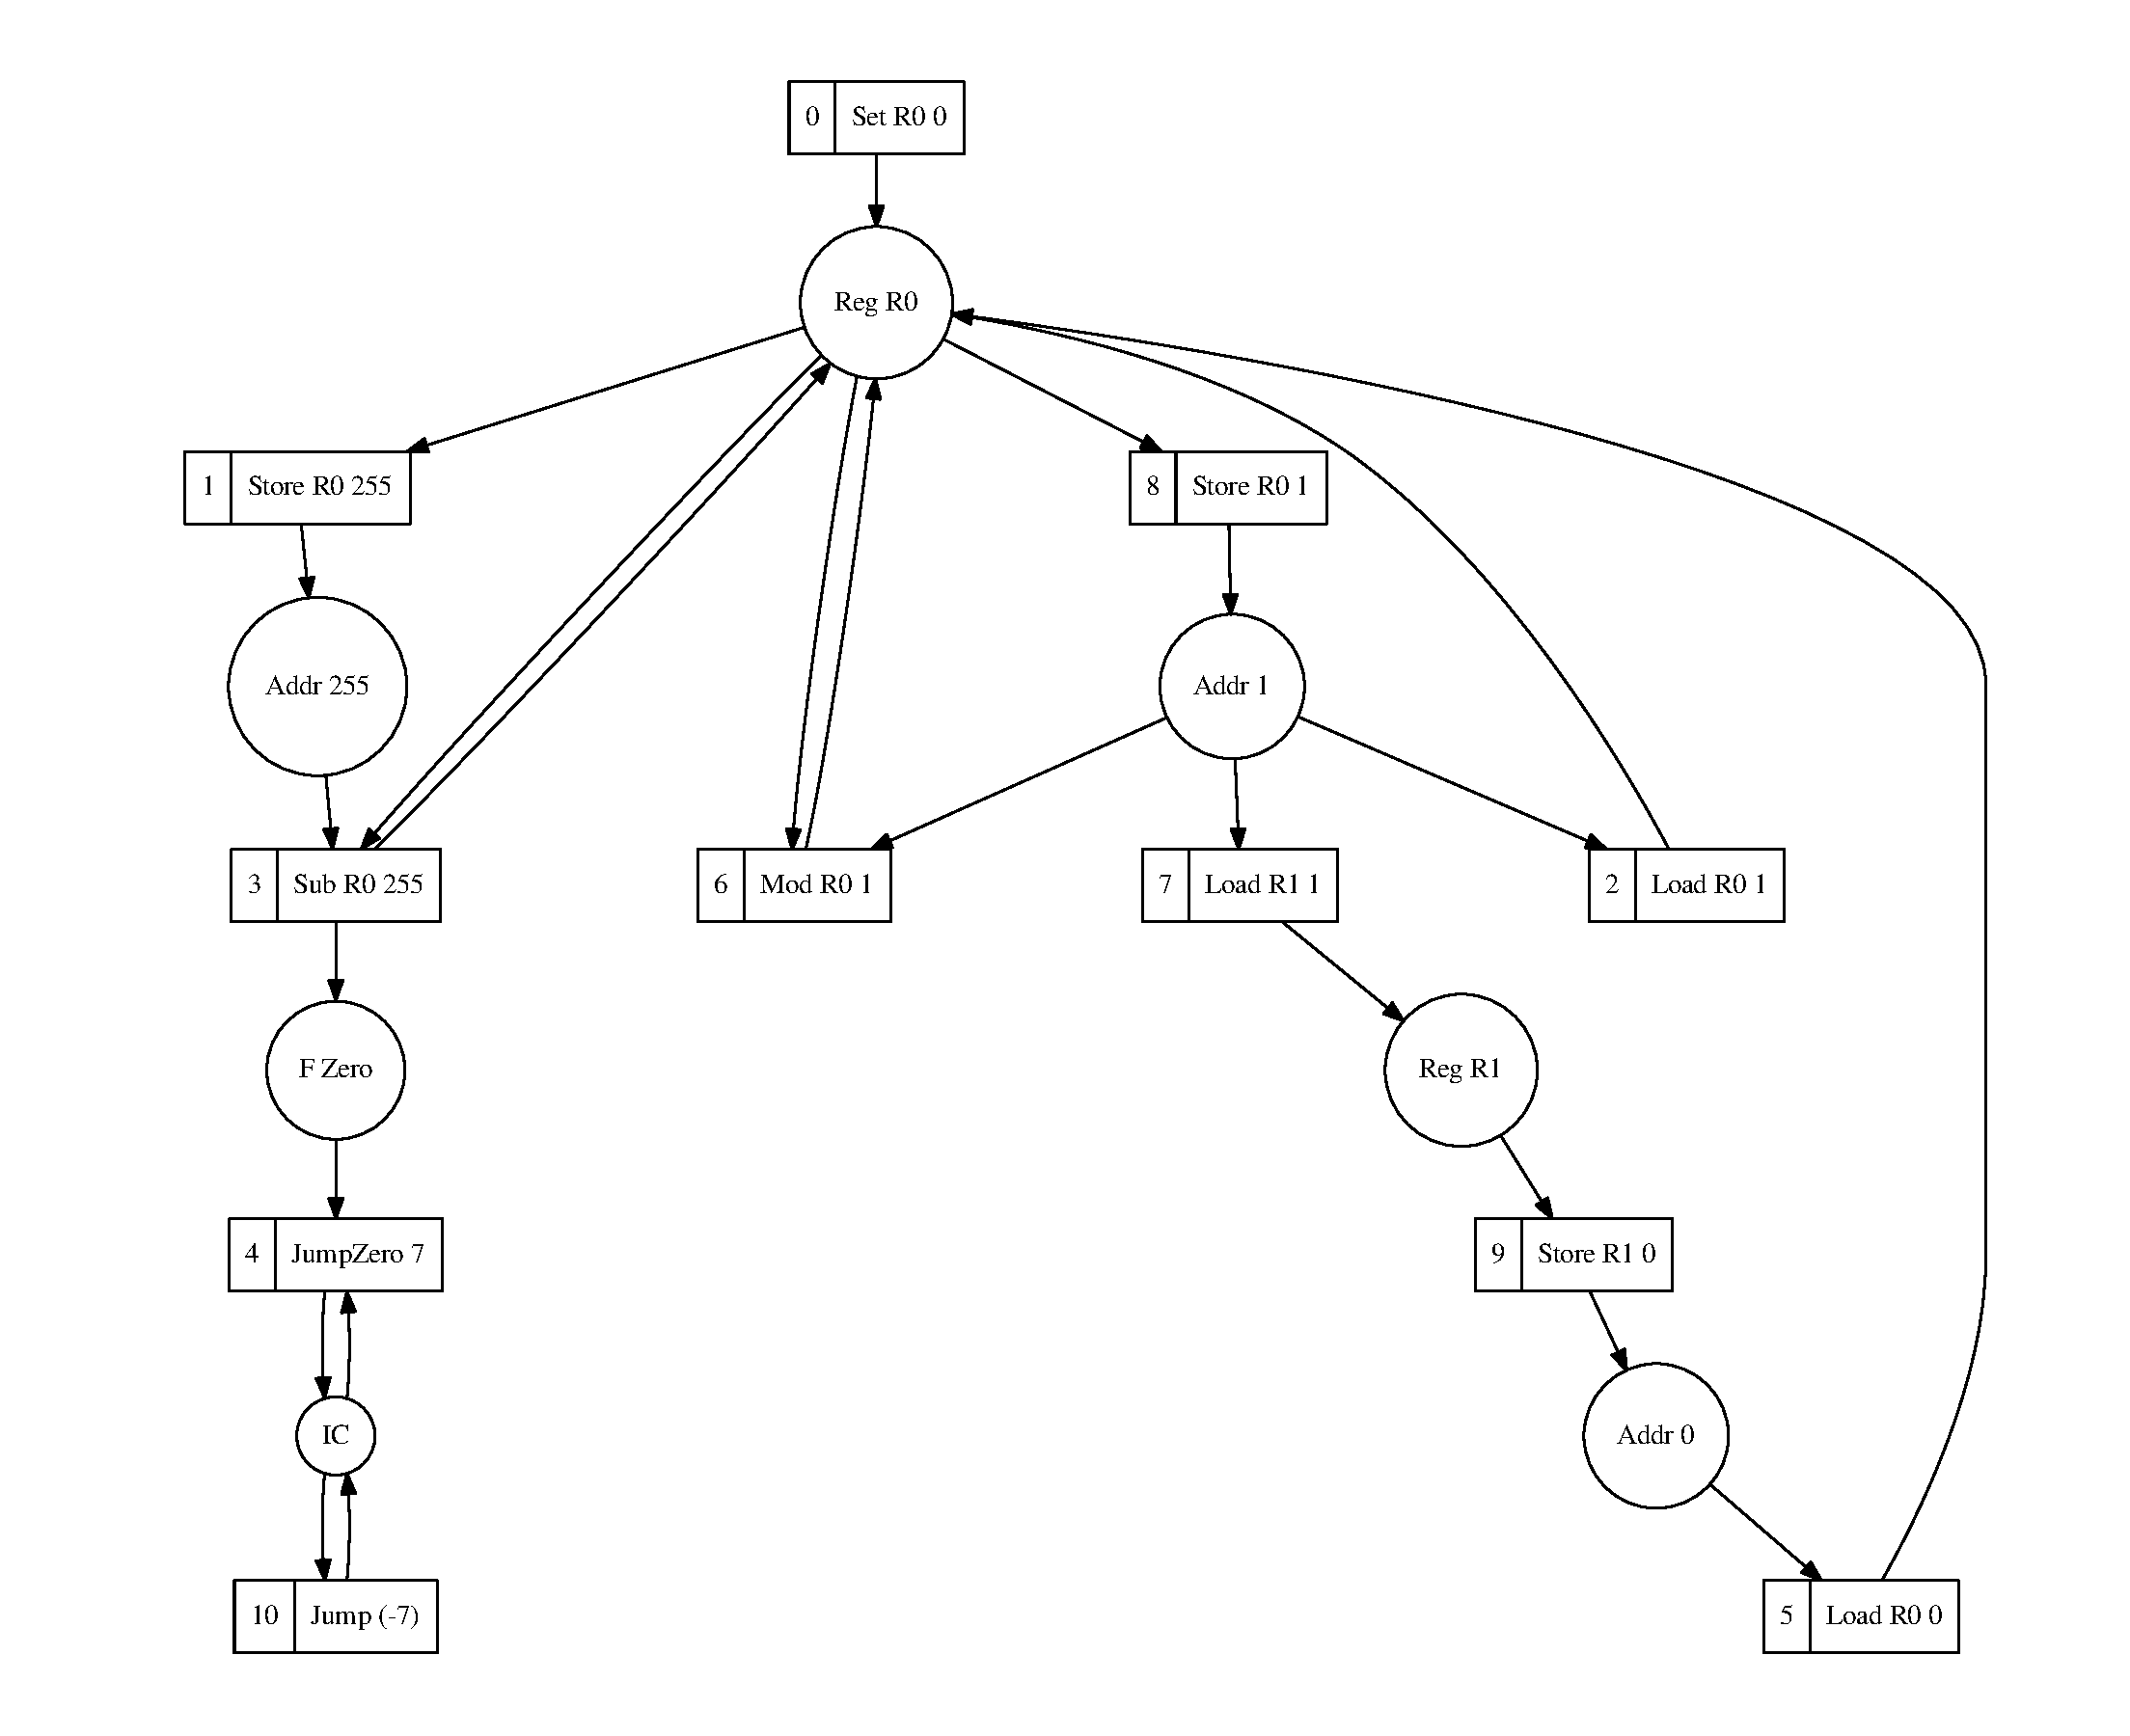
\includegraphics[scale=0.4]{img/gcd.pdf}}
\vspace{-7mm}
\caption{Approximation of static dependencies of the Euclidean algorithm.\label{fig-sum}}
\vspace{-10mm}
\end{figure}
% \clearpage

%
% ---- Bibliography ----
%
% BibTeX users should specify bibliography style 'splncs04'.
% References will then be sorted and formatted in the correct style.
%
\bibliography{biblio}
\end{document}
